\documentclass[nonatbib,preprint,12pt,authoryear]{elsarticle}
\usepackage{graphicx} % Required for inserting images
\usepackage{amssymb}
\usepackage{lipsum}
\usepackage{booktabs}
\usepackage{array,longtable}
\usepackage[utf8]{inputenc}
\usepackage[T1]{fontenc}
%\usepackage[table]{xcolor}
\usepackage{amsfonts, amssymb, amsthm, mathrsfs,amscd,bezier, amsfonts,latexsym}
\usepackage{mathtools, nccmath}
\usepackage{amsmath}
\usepackage{bbold}
\usepackage{MnSymbol}
\usepackage[all]{xy}
\usepackage{stmaryrd}
\usepackage{csquotes}
\usepackage{float}
\usepackage{indentfirst}
\usepackage{tabularx}
\usepackage{geometry}
\usepackage[hidelinks]{hyperref}
\usepackage{comment}
\usepackage[Algoritmo]{algorithm}
\usepackage{listings}
\usepackage{datetime2}
\usepackage{algorithmic}
\usepackage{subfigure}
\usepackage{caption}
\usepackage{subcaption}
%\usepackage[nottoc,numbib]{tocbibind}
\usepackage{enumitem}
\usepackage{xcolor}

\usepackage{amsmath}
\usepackage{tikz}
\usepackage{mathdots}
\usepackage{yhmath}
\usepackage{cancel}
\usepackage{color}
\usepackage{siunitx}
\usepackage{multirow}
\usepackage{amssymb}
\usepackage{gensymb}
\usepackage{extarrows}
% \usepackage{natbib}

\journal{Journal: To be precised}

\begin{document}

\begin{frontmatter}
\title{Bayesian sampling algorithms comparison for deterministic ODE-based Infectious Disease models}
\tnotetext[t1]{This study was supported by the French government through the program "\textit{France 2030}" (SFRI project GRAEL/ ANR-21-SFRI-005) managed by the National Research Agency.}

%% use optional labels to link authors explicitly to addresses:
%% \author[label1,label2]{}
%% \affiliation[label1]{organization={},
%%             addressline={},
%%             city={},
%%             postcode={},
%%             state={},
%%             country={}}
%%
%% \affiliation[label2]{organization={},
%%             addressline={},
%%             city={},
%%             postcode={},
%%             state={},
%%             country={}}

\author[University of Lille]{Abdoul Aziz Diallo}
\ead{abdoul-aziz.diallo@univ-lille.fr}
\affiliation[University of Lille]{organization={Department Mathematics, University of Lille},%Department and Organization
            %addressline={V}, 
            city={Villeneuve d'Ascq},
            postcode={59650}, 
            state={Hauts de France},
            country={France}}

\author[Monash University]{Romain Ragonnet}

\affiliation[Monash University]{organization={Epidemiological Modeling Unit, Department of Epidemiology and Preventive Medicine
School of Public Health and Preventive Medicine, Monash University},%Department and Organization
            addressline={553 St Kilda Rd}, 
            city={Melbourne},
            postcode={3004}, 
            state={Victoria},
            country={Australia}}
\author[James Cook University]{Alec Henderson}

\affiliation[James Cook University]{organization={Australian Institute of Tropical Health and Medicine, James Cook University},%Department and Organization
%addressline={553 Saint Kilda Road}, 
            city={Townsville},
            %postcode={3004}, 
            %state={Victoria},
            country={Australia}}

\begin{abstract}
 Model fitting and calibration are crucial yet challenging tasks in infectious disease modeling, particularly in high-dimensional problems. Bayesian sampling methods offer a robust framework for automatic calibration. However, these techniques come with their own set of challenges, especially for complex models. The performance of Bayesian sampling algorithms can vary significantly based on the problem’s characteristics, and because these methods aim to approximate distributions asymptotically, characterizing convergence becomes complex.

 In this paper, we compare the performance of five Bayesian sampling algorithms across different ODE-based Infectious Disease Models. The pseudo-convergence phenomena was illustrated using a synthetic bimodal posterior. 
\end{abstract}
\newpageafter{abstract}

%%Graphical abstract
% \begin{graphicalabstract}
% \includegraphics{grabs}
% \end{graphicalabstract}

%%Research highlights
\begin{highlights}
\item Research highlight 1
\item Research highlight 2
\end{highlights}

\begin{keyword}
%% keywords here, in the form: keyword \sep keyword
Infectious Disease Modelling \sep Bayesian sampling\sep Markov Chain Monte Carlo \sep Ordinary Differential Equations
%% PACS codes here, in the form: \PACS code \sep code
%\PACS 0000 \sep 1111
%% MSC codes here, in the form: \MSC code \sep code
%% or \MSC[2008] code \sep code (2000 is the default)
%\MSC 0000 \sep 1111
\end{keyword}

\end{frontmatter}

\section{Introduction}
\label{sec:MCMC_Compar_Intro}
The spread of an infectious disease can be studied by mean of mathematical models. Deterministic Ordinary Differential Equation (ODE) are widely used for this purpose. These models can provide valuable insights into the dynamics of disease transmission and the effects of various interventions. 
The fitting or calibration phase in the modelling process is crucial and challenging specially in high dimensional problems.

Techniques such as Markov Chain Monte Carlo (MCMC) using Bayesian inference are developed to overcome this challenge. Recent research highlights an increasing application of MCMC methods to calibrate ODE-based models of infectious diseases to empirical data. For instance, in \cite{wang_data-driven_2013}Wang et al. utilized the adaptive Metropolis algorithm to calibrate a SEIS deterministic model using time series data. Similarly, Hauser et al. employed Hamiltonian Monte Carlo algorithm in \cite{hauser_counotte_margossian_konstantinoudis_low_althaus_riou_2020} to estimate their model's parameters.

However, employing MCMC techniques presents its own set of challenges, particularly for complex models. The performance of these algorithms can vary significantly depending on the characteristics of the problem at hand. Additionally, MCMC methods aim to approximate a distribution asymptotically, which complicates the notion of convergence and makes it difficult to characterize precisely. The metrics developed to diagnose MCMC convergence may not always be reliable, as highlighted by Cowles and Carlin \cite{cowles_markov_1996}.

To date, we are aware of relatively few studies that have focused on comparing MCMC algorithms specifically for inferring parameters in deterministic ODE-based infectious disease models. Li et al. \cite{li_fitting_2018} examined the fitting efficiency of various platforms, including JAGS, NIMBLE, and STAN (using Hamiltonian Monte Carlo). Meanwhile, Chatzilena et al. \cite{chatzilena_contemporary_2019} explored the fitting of different epidemic models, including the basic SIR model and a multi-strain SIR model, using Hamiltonian Monte Carlo and variational inference. Their study primarily focused on the models, inference methods and platforms rather than a direct comparison of MCMC algorithms.

This work focus on comparing some MCMC algorithms implemented in PyMC and the No-U-Turn Sampler (NUTS) from numpyro. The ODE-based ID models are built and solved by the \textit{Summer/Estival} packages developed by the Epidemiological Modelling Unit(\href{https://www.monash.edu/medicine/sphpm/units/epidemiological-modelling}{\textcolor{blue}{EMU}}) team of Monash Public Health and Preventive Medicine.
We first describe in \ref{sec:Material_Methods} the MCMC calibration approach using Bayesian inference. This is followed by an exploration of its application across various problems: fitting a simple SIR model to dummy data, calibrating an age-stratified model using daily COVID-19 case counts from England in 2020, and addressing a reverse engineering problem involving a mixture of two Gaussian distributions for the contact rate parameter in the SIR model.

\section{Materials and Methods}
\label{sec:Material_Methods}
\subsection{Markov chain Monte Carlo sampling using Pymc and Numpyro}
The MCMC algorithms aim to estimate a \textbf{posterior} distribution for purpose of inference.
Given a probability distribution, one can construct a Markov chain whose stationary distribution approximates this target distribution. Specifically, the equilibrium distribution of the Markov chain will converge to the desired distribution. Theoretically, as the number of steps in the Markov chain increases, the sample distribution more closely matches the target distribution \cite{padmanabhan_ranjan_2022_Markov_Chain}.
In our situation, we want to estimate the posterior distribution of the model's parameters which better describe our observations. This calibration process aims to respond the following question: Given data ($Y = (y_i)_i$) and prior knowledge about the parameters, what values should take these parameters such the model is capable to capture the empirical observations? 
Bayes theorem helps us to formulate this problem. Therefore given the observation $Y$, the posterior distribution $\mathbb{P}(\theta \mid Y) $ of the set of parameters $\theta$ is given by:

\begin{equation}
    \label{eq:poste_bayes_thrm}
    \mathbb{P}(\theta \mid Y) = \frac{\mathbb{P}(Y \mid \theta) \times \mathbb{P}(\theta)}{P(Y)}
\end{equation}
$\mathbb{P}(Y \mid \theta)$ is the Likelihood distribution which quantify the quality of simulating the observed data by the model given the parameter set $\theta$, whereas $\mathbb{P}(\theta)$ is the prior distribution of $\theta$, it helps incorporating prior knowledge or beliefs of the calibrated parameters.\\
$\mathbb{P}(Y) = \int \mathbb{P}(Y \mid \theta) \times \mathbb{P}(\theta)$ is The normalizing constant, whose computation can become computationally intensive, particularly in high-dimensional settings.
The Figure (\ref{fig:Posterior}) describes the posterior computation process.
\begin{figure}[H]
    \centering
    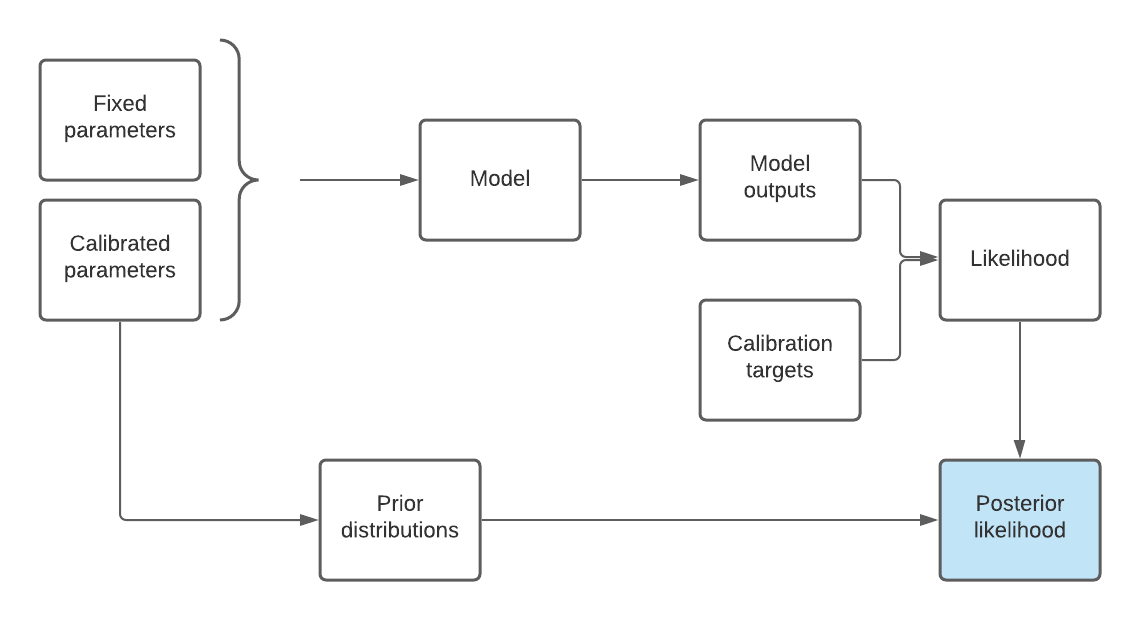
\includegraphics[width = 0.8\linewidth, height = 0.5\linewidth]{Figures/posterior_computation_overview.png}
    \caption{Overview of posterior computation}
    \label{fig:Posterior}
\end{figure}
 MCMC is a set of numerical approach to estimate $\mathbb{P}(\theta \mid Y)$ avoiding the computation of $\mathbb{P}(\theta)$.

The key feature using Bayesian sampling approach is the ability to account for parameter uncertainty. Instead of providing a single optimal set of parameters, this approach offers a range of plausible parameter configurations that collectively represent the observed data. This comprehensive set of parameter values reflects the uncertainty in the estimates and captures the variability in the model's predictions. This is particularly valuable because real-world data often contain noise and variability, and a single "best fit" parameter set may not adequately capture this variability or the inherent uncertainty.% in our knowledge.

PyMC \cite{pymc2023} is a Python library dedicated to probabilistic programming, specifically designed for Bayesian modelling and inference using MCMC methods. It offers a high-level interface that allows users to define complex probabilistic models and perform Bayesian inference efficiently.

Similarly, NumPyro \cite{bingham2019pyro} \cite{phan2019composable} leverages the power of JAX for high-performance numerical computing and automatic differentiation. This combination enables NumPyro to compute gradients of probabilistic models seamlessly, facilitating the implementation of efficient gradient-based inference algorithms such as Hamiltonian Monte Carlo (HMC).

Both PyMC and NumPyro provide flexible frameworks for specifying Bayesian models, conducting inference, and analyzing results. While PyMC is established within the Python Bayesian community for its intuitive syntax and MCMC capabilities, NumPyro offers a modern alternative with enhanced performance and scalability through JAX.

Furthermore, while tuning MCMC algorithms hyper-parameters is tough challenging, both PyMC and Numpyro offer a efficient way to handle it. Tuning or warm-up are crucial in the sampling process. Broadly, they describe what happen before sampling, adjusting parameters such as step sizes, acceptance rates, and scaling factors. The number of tuning samples can be discarded, in other words they can be considered as a \textit{burn-in} period which refers theoretically to the number of samples after which the new generated samples comes asymptotically from the stationary distribution \footnote{\href{https://colcarroll.github.io/hmc_tuning_talk/}{Tuning Talk in PyMC3}} 

In this work, we have constructed and executed a Bayesian compartmental model using the Summer package. This model can be seamlessly implemented and utilized in either PyMC, leveraging its MCMC algorithms, or in NumPyro, taking advantage of JAX for efficient gradient-based inference.

The Summer package enables a flexible approach to transitioning between platforms without the need for extensive customization of the model and settings. This adaptability is crucial for exploring different inference and optimisation methods and optimising computational performance across varying computational frameworks. 

In this paper, the inference algorithms we use are the Metropolis-Hastings(often called Random Walk Metropolis RWM), the Differential Evolution Metropolis(DE-MC and DE-MCz), the No-U-Turn Sampler (NUTS) and the Sequential Monte Carlo (SMC). 
The output of these algorithms is a sample $(\theta^1, \theta^2, \ldots, \theta^n)$ from a stationary distribution $\pi(\theta)$ such that $\pi(\theta) = \mathbb{P}(\theta \mid Y)$ where $n$ is the number of draws. 

\subsubsection{The Metropolis-Hasting :}The Metropolis-Hasting algorithm is the simplest version of MCMCs. The algorithm begins by establishing a Markov process through defined transition probabilities $T(\theta^{i+1} \mid \theta^i)$, the probability of transitioning from the state $\theta^i$ to the state $\theta^{i+1}$. The algorithm's derivation initiates with the requirement of detailed balance condition which is a sufficient condition ensuring the existence of $\pi(\theta)$ \cite{padmanabhan_ranjan_2022_Markov_Chain} which is chosen to match the posterior distribution $\mathbb{P}(\theta \mid Y)$.
\begin{equation}
    \label{eq:Detailed_Balanced_Condition}
    \pi(\theta^i) T(\theta^{i+1} \mid \theta^i) = \pi(\theta^{i+1}) T(\theta^i \mid \theta^{i+1})
\end{equation}
Following this the transition probability is then split in two components : a proposal distribution $g(\theta^{i+1} \mid \theta^i)$ and a acceptation probability $A(\theta^{i+1},\theta^i)$.
$$T(\theta^{i+1} \mid \theta^i) = A(\theta^{i+1},\theta^i) \times g(\theta^{i+1} \mid \theta^i) $$
The detailed balanced condition become then
$$ \pi(\theta^i) \times A(\theta^{i+1},\theta^i) \times g(\theta^{i+1} \mid \theta^i) = \pi(\theta^{i+1}) A(\theta^i \mid \theta^{i+1}) \times g(\theta^i \mid \theta^{i+1}) $$ and can be rewritten as
$$\dfrac{A(\theta^{i+1},\theta^i)}{A(\theta^i,\theta^{i+1})}= \dfrac{g(\theta^i \mid \theta^{i+1}) \times \pi(\theta^{i+1})}{g(\theta^{i+1} \mid \theta^i) \times \pi(\theta^i)}$$
Since $\pi(\theta)$ is chosen to match the posterior $\mathbb{P}(\theta \mid Y) $ it can be replaced by \ref{eq:poste_bayes_thrm}. The interesting thing using this Bayes expression of the posterior is the fact that the normalizing constant is cancel out in the acceptation probability computation. Only the prior and the likelihood are involved.
$$\dfrac{A(\theta^{i+1},\theta^i)}{A(\theta^i,\theta^{i+1})}= \dfrac{g(\theta^i \mid \theta^{i+1}) \times \mathbb{P}(Y \mid \theta^{i+1}) \times \mathbb{P}(\theta^{i+1})}{g(\theta^{i+1} \mid \theta^i) \times \mathbb{P}(Y\mid \theta^i) \times \mathbb{P}(\theta^i)}$$
The following Metropolis acceptance probability ensure the detailed balanced condition.
\begin{equation}
    \label{eq:Metropolis_ratio}
    A(\theta^{i+1},\theta^i) = \min (1, H)
\end{equation}
Where $H = \dfrac{g(\theta^i \mid \theta^{i+1}) \times \mathbb{P}(Y \mid \theta^{i+1}) \times \mathbb{P}(\theta^{i+1})}{g(\theta^{i+1} \mid \theta^i) \times \mathbb{P}(Y\mid \theta^i) \times \mathbb{P}(\theta^i)}$ is called the Hasting ratio.
A random candidate $\theta^{i+1}$ is generated randomly according to the proposal distribution $g$ and a jump to this state is performed under the probability $A$.

Provided that, the Metropolis Hasting algorithm help to explore the parameter space and asymptotically converge to the posterior.

\subsubsection{The Differential Evolution Markov Chain :}
The Differential Evolution Metropolis (DE-MC) algorithm combines Differential Evolution (DE), a meta-heuristic optimization technique, with the Metropolis-Hastings (MH) algorithm to enhance sampling efficiency from probability distributions \cite{ter_braak_differential_2008}. This hybrid approach leverages DE's global search capabilities to improve exploration and exploitation of the parameter space.

In DE-MC, $N$ parallel chains, representing the population, are run. The update for the state $\theta_i$ of the $i$-th chain involves generating a proposed candidate $\theta_p$, which is a $d$-dimensional vector, using the following equation:
$$\theta_p = \theta_i + \gamma(\theta_{R_1} - \theta_{R_2}) + e$$
Here, $\theta_{R_1}$ and $\theta_{R_2}$ are randomly selected from the remaining $N-1$ chains (excluding the current chain $i$), and $e$ is drawn from a symmetric distribution. The proposal $\theta_p$ is then accepted based on the Metropolis acceptance probability, without reference to the proposal distribution.

The standard DE-MC algorithm requires that $N$ exceeds $d$ (the dimensionality of the parameter space). Therefore despite its recognized efficiency, the method can be challenging to apply in high-dimensional spaces \cite{ter_braak_differential_2008}. To address this issue, Cajo J.F. ter Braak and Jasper A. Vrugt extended the DE-MC algorithm to DE-MCz. This extension, where 'z' refers to the introduction of a matrix $Z$ that includes the current and past states of the chains, allows for effective sampling in high dimensions with fewer chains. In DE-MCz,the difference vectors are sampled from the past states of the chains. 
Roughly speaking DE-MC may not be considered typically as a proper Markov Chain, since current sampled states rely on past states of the different chains even though they are chains states are designed to be independent asymptotically \cite{braak_markov_2006}. 

Both versions of the algorithm are implemented efficiently in PyMC and their performance has been compared in \cite{Pymc_DEM_DEMz_comparison}

\subsubsection{The No-U-Turn Sampler :}
Hamiltonian Monte Carlo (HMC) is a gradient-based MCMC method that leverages Hamiltonian dynamics to generate more distant proposals than the Metropolis algorithm. This approach helps overcome the slow exploration of the state space often encountered with the diffusive nature of basic random-walk proposals \cite{Brooks_NEAL_HMC_2011}. HMC achieves this by transforming the posterior density into a potential energy function and introducing "momentum" variables alongside the parameters of interest, which are treated as "position" variables. This enables HMC to efficiently explore complex, high-dimensional distributions and reduce sample correlations.

Despite its strengths, HMC presents challenges in the selection of the step size $\epsilon$ and the number of integration steps $L$ required for the leapfrog method to discretize the Hamiltonian equations \cite{Brooks_NEAL_HMC_2011}, \cite{hoffman_no-u-turn_2014}. To address these issues, the No-U-Turn Sampler (NUTS) extends HMC by eliminating the need for manual tuning of these parameters \cite{hoffman_no-u-turn_2014}. NUTS automatically adapts the trajectory length, making it a more practical and efficient implementation of HMC.

The NUTS is one of the most commonly used MCMC in Numpyro \cite{phan2019composable}. In the Numpyro NUTS, the step size and the mass matrix used as the covariance matrix of the distribution to sample the momentum variables, can be efficiently adapted during the warm-up phase of the algorithm according to the acceptance probability. 

Furthermore, since initialization is crucial for exploration, NumPyro offers various initialization strategies that users can experiment with to achieve efficient exploration. It is possible too, to manually initialise parameters for each chain.

\subsubsection{Sequential Monte Carlo Chain (SMC):} Sequential Monte Carlo (SMC) methods are a set of simulation-based techniques designed for efficiently computing posterior distributions, particularly in dynamic or sequential settings\cite{Doucet2001_SMC_Intro,KANTAS2009774_SMC_Overview}.
The SMC implemented in PyMC use transitioning to overcome the difficulty to sample from multi-peaked posterior distribution combining tempering, importance sampling and the Metropolis Hasting approach \footnote{\href{https://www.pymc.io/projects/examples/en/latest/samplers/SMC2_gaussians.html}{"Sequential Monte Carlo". In: PyMC Examples. Ed. by PyMC Team.}} \cite{minson_bayesian_2013_TMCMC,Transitional_MCMC}. Instead of sampling directly from the posterior, an auxiliary distribution $\mathbb{P}(\theta \mid Y)_\beta $ controlled by a temperature parameter $\beta \in [0,1]$ is sampled from. 
$$\mathbb{P}(\theta \mid Y)_\beta = \mathbb{P}(Y \mid \theta)^\beta \times \mathbb{P}(\theta) $$
The algorithm begins by sampling from the prior ($\beta = 0$) and when $\beta = 1$ it reaches its final stage with samples from the true posterior(based on the previous relation).

In each stage of the algorithm, $N$ independent Metropolis-Hastings steps are performed, each starting from different weighted samples. 

The value of $\beta$ in SMC is determined dynamically based on the characteristics of the posterior distribution. If the posterior is challenging to sample from, transitions tend to be smaller, leading to a higher number of stages. The progression of $\beta$ values can be manually adjusted using the \textit{threshold} and \textit{correlation threshold} parameters (see \href{https://www.pymc.io/projects/docs/en/latest/api/generated/pymc.smc.sample_smc.html}{\textcolor{blue}{documentations}}).

The tempering approach, which is a crucial component of SMC, has been extensively discussed in \cite{Brooks_NEAL_HMC_2011}. It improves the performance of Hamiltonian Monte Carlo (HMC) when dealing with distributions that have separated modes.

\subsection{Modeling}
\subsubsection{The SIR model:}
Deterministic ODE-based models are widely used in Infectious disease modeling. The Susceptible Infectious Recovered (SIR) model is the simplest one that can describe the dynamic of an infectious disease. This model has been used in \cite{chatzilena_contemporary_2019} for statistical inference comparison. In this framework the population size is split into compartments (Susceptible, Infectious, Recovered) and the flows (the variation of each compartment size over the time) between these compartment is tracked by mean of ordinary differential equations. Therefore this model aims to predict the number of individuals who are susceptible to infection, are actively infected, or have recovered from infection at any given time \cite{bjornstad_on_modeling_2020}.

Let's denote $\dfrac{dX(t)}{dt}$ by $\Dot{X}(t)$(the variation of the size of the compartment$X$ over the time $t$).

\begin{equation}
    \label{eq:SIR_article}
    \left\{\begin{array}{rcl} 
        \Dot{S}(t) &=& -\beta \cdot \dfrac{S(t) \cdot I(t)}{N}, \\
        \Dot{I}(t) &=& \beta \cdot \dfrac{S(t) \cdot I(t)}{N} - \gamma \cdot I(t), \\
        \Dot{R}(t) &=& \gamma \cdot I(t)
    \end{array}\right.
    \end{equation}
$N = S(t) + I(t) + R(t)$ represents the total population size. Given the initial population setting $S(0), I(0)$ and $R(0)$, the dynamic of the disease is driven by the two key parameters $\mathbf{\beta}$ and $\mathbf{\gamma}$.
The parameter $\beta$ is defined as the \textit{\textbf{per capita}} rate at which susceptible individual and infectious individual come into effective contact per unit of time\cite{vynnycky2010introduction}. 
Therefore the risk of infection at time $t$ can be expressed as:
$$ \lambda(t) = \beta \cdot I(t)$$
It depends in many factors such as the involved disease, the character and  behavior of the studied population and so on. For the seek of simplicity, we suppose here an homogeneous transmission of the disease among the population (random or homogeneous mixing) and constant values for the parameters over the time.

$\mathbf{\gamma}$ represents the rate at which infectious individuals recover per unit unit of time. It describes the intensity at which go to compartment \textbf{R} to the compartment \textbf{I} at time $t$.

The main challenge of infectious disease modeling is to obtain reliable values estimate of these parameters. Note that the population initial state can be estimated too. 
However we limit ourselves in this presentation to the estimation of $\mathbf{\beta}$ and  $\mathbf{\gamma}$.

To obtain estimates through Bayesian Inference using MCMC sampling techniques, we fit the model to daily cases of infections. A uniform prior is chosen for all parameters.

$$\beta \sim \mathcal{U}(0,1)$$ $$\gamma \sim \mathcal{U}(0,1   )$$

For this model we generate dummy data representing daily active cases. The $N$ data points were deliberately chosen to mimic a bell-shaped curve, which is characteristic of many infectious disease outbreaks. 
We choose a normal distribution to define the likelihood probability distribution:
$$y_i \sim \mathcal{N}(x_i^\theta, \sigma)$$
$$\mathcal{L}(\theta) = \prod_{i=1}^N f_{y_i}(\theta, x_i)$$
$f_{y_i}(\theta, x_i)$ is the probability density of $\mathcal{N}(x_i^\theta, \sigma)$
\subsubsection{The SEIR age-stratified:}
Even though the basic SIR deterministic model is a powerful approach to understand infectious disease dynamic over a random-mixing population, complex models such Susceptible-Exposed-Infected-Recovered (SEIR) can capture very complex features. Here we build an SEIR age-stratified model to highlight the age-dependant effects in the transmission. In other words this allows us to analyze how the transmission factors vary across different age groups within the population. This model can be seen as an simplification of the one developed in  \cite{davies_age-dependent_2020}. We suppose an homogeneous incubation period $\sigma$ and an infectious period $\gamma$ across the whole population. Furthermore, we assume that individuals for all age groups have equal probability of coming into contact with infectious individuals. This implies a uniform mixing between age groups and therefore a contact matrix is not needed. 
The following (\ref{eq:SEIR_age-stratified}) system of ODEs describe the mathematical model.
\begin{equation}
    \label{eq:SEIR_age-stratified}
    \left\{\begin{array}{rcl} 
        \Dot{S}_i &=& -\beta_i \cdot S_i \cdot \sum_j\dfrac{I_j}{N_j}, \\
        \Dot{E}_i &=& \beta_i \cdot S_i \cdot \sum_j\dfrac{I_j}{N_j} - \sigma E_i\\
        \Dot{I}_i &=&  \sigma \cdot E_i - \gamma \cdot I_i, \\
        \Dot{R_i} &=& \gamma \cdot I_i
    \end{array}\right.
    \end{equation}
Where $N_i$ and $\beta_i$ are respectively the population size and the transmission rate in the age group $i$ and we have $\sum_i N_i = N$ the total population.
We fit our model to daily cases counted in England extracted from the  \href{https://ukhsa-dashboard.data.gov.uk/covid-19-archive-data-download}{\textcolor{blue}{decommissioned Coronavirus in the UK dashboard}}. The considered age categories are: 
\begin{itemize}
    \item 0 : $00-04$ years;
    \item 5 : $05-09$;
    \item $\ldots$ 
    \item 60 : 60 and above; 
\end{itemize}
The population size for these categories is based on the \href{https://www.ons.gov.uk/datasets/TS007/editions/2021/versions/3/filter-outputs/5c265388-33f5-4c92-a6de-bb7f220afb63#get-data}{\textcolor{blue}{Census 2021 estimates}} of usual residents in England. The Figure \ref{fig:total_case_UK} shows the total counted cases by age group over the period June $2020$ - December $2020$. 

A uniform prior is chosen for all transmission rates $\beta_i$ whereas a the incubation and infectious periods were fixed.
$$\beta_i \sim \mathcal{U}(0,0.8)$$
$$\sigma  = 5.4 , \gamma = 7.3~~\text{(Reference: \cite{chen_lau_xu_wang_du_tsang_wu_lau_wallinga_cowling_2022})}$$

We also calibrated the seed $I(0)$ and the initial susceptible population $S_0$ whereas $R(0)$ and $E(0)$ are fixed to zero.
We introduce a case detection rate which is indeed calibrated to allow more flexibility and reality on the model, as not all cases are detected during the outbreak. Uniform priors were also chosen for these parameters.

\begin{figure}[H]
    \centering
    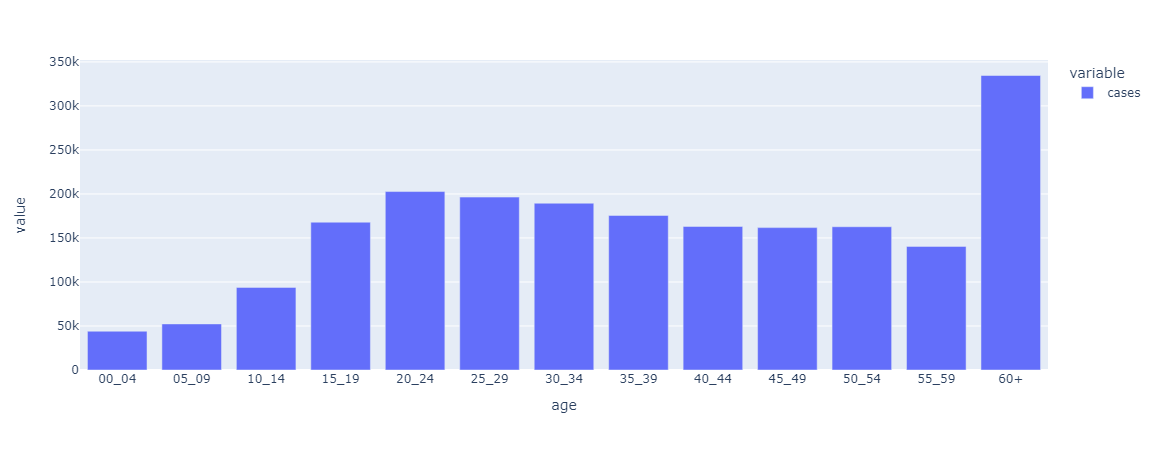
\includegraphics[width=\linewidth]{Figures/Model_2/England_covid_total_cases_08-to-12-2020.png}
    \caption{Total cases number of COVID in England by age group during the period June $2020$ to December $2020$ (Source: \href{https://ukhsa-dashboard.data.gov.uk/covid-19-archive-data-download}{\textcolor{blue}{UK COVID dashboard}) } }
    \label{fig:total_case_UK}
\end{figure}

\subsubsection{Reverse Engineering:} 
In this final experiment, we examine the performance of various MCMC samplers when dealing with bimodal posterior distributions that could arise in Infectious disease modelling.
Specially, we sample a bimodal normal distribution-say a mixture of two normal distributions-for the transmission rate $\beta$ in the SIR model. We therefore run the SIR model through those samples to obtains synthetic data which are used to build a likelihood for the Bayesian inference. Since we know the true posterior distribution in this controlled setup, we can evaluate how well different MCMC algorithms recover it. We investigate here which of these MCMC algorithms mentioned above could help to perform this task.
\begin{figure}[H]
    \centering
    %\begin{subfigure}
    %\centering
    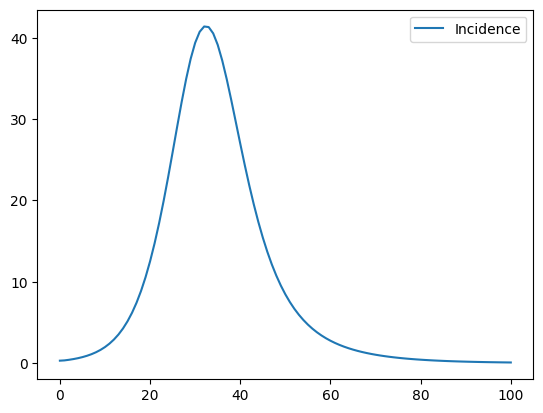
\includegraphics[width = 0.68\linewidth, height = 5cm]{Figures/Reverse-Ingineering/Model_output.png}
    \caption{SIR Model's output.}
    \label{fig:SIR_reverse_Engi_output}
    %\end{subfigure}%
\end{figure}
    %\hspace{0.5em}
\begin{figure}[H]
    \centering
    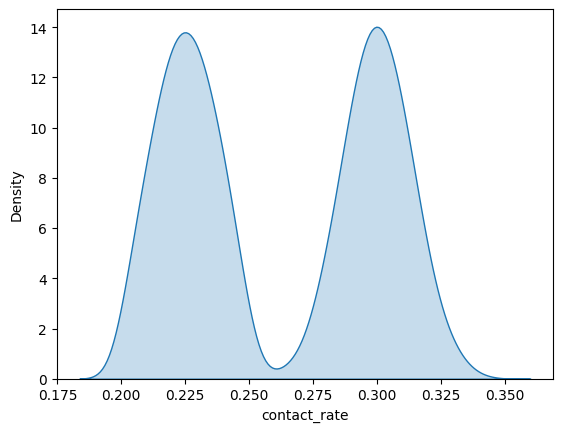
\includegraphics[width = 0.7\linewidth, height = 5cm]{Figures/Reverse-Ingineering/True_posterior.png}
    \caption{Synthetic Posterior distribution of $\beta$}
    \label{fig:True_sample_with_junction}
    \label{fig:Reverse_Ingineering_output_posterior}
\end{figure}

\subsection{Convergence diagnostics}
The term convergence in the world of MCMC sampling is quite subtle, even though several metrics have been developed to characterize it. Cowles et al. provided a good review of these metrics and their applicability \cite{cowles_markov_1996}.  
The most common practical technique is the \textit{multi-start heuristic}. It corresponds running multiple independent chains starting eventually at different points of the space and tracking if they all converge towards the same equilibrium. The Gelman and Rubin $\mathbf{\hat{R}}$ is designed  monitoring convergence of multiple chains alongside the \textbf{Effective Sample Size} (\cite{vehtari_rank-normalization_2021}, \cite{cowles_markov_1996}). The Monte Carlo Standard Error statistics (MCSE) which measure the variability or uncertainty in the estimate  obtained by a MCMC is also very useful to assess the parameter approximation accuracy. 


\begin{itemize}
     \item \textbf{Gelman and Rubin ($\hat{R}$)} : The $\hat{R}$ statistic is the ratio of the average variance within each individual chain to the variance of the combined samples across all chains. If the chains are mixing well that is they all converge to the same distribution, $\hat{R}$  will be equal to one and conversely will exceed one in the poor mixing situation.
     \item \textbf{Effective Sample Size (ESS)} : The effective sample size is a measures of the independent draws which would contain the same amount of information as the dependent sample obtained by the MCMC algorithm \cite{vehtari_rank-normalization_2021}. A high value of the Ess is expected for a good  chains convergence. The standard Ess is estimated following the \href{https://mc-stan.org/docs/2_18/reference-manual/effective-sample-size-section.html#definition-of-effective-sample-size}{\textcolor{blue}{Stan Development Team description}}. Moreover, Vehtari et al \cite{vehtari_rank-normalization_2021}, proposed another estimates of the ESS including and between-chain variance in the computation. 
\end{itemize}
In addition of these metrics, a visual diagnostic is also crucial while dealing with MCMC sampling. Indeed, the trace of each chain across the iterations can be visualized in order to detect good or bad mixing chains. Vehtari et al \cite{vehtari_rank-normalization_2021} suggest to use rank plots instead of the trace plots from multiple chains. If all MCMC chains are sampling from the same posterior distribution, we expect the ranks within each chain to be uniformly distributed. Deviations from uniformity suggest that one or more chains might be targeting different locations or scales. Unlike trace plots, rank plots maintain clarity and are less likely to become cluttered with long chains.

To carry out our convergence diagnostics, we use the famous and powerful \href{https://python.arviz.org/en/stable/}{\textcolor{blue}{Arviz python package}} which supports a variety of metrics (ESS, $\hat{R}$, MCSE,...) and plots (trace plots, rank plots, pair plot,...).
\begin{itemize}
    \item \textbf{Kullback-Leibler Divergence (KL\textunderscore div)}: In our reverse engineering experiment, convergence of sampling methods can be effectively characterized by monitoring the Kullback-Leibler divergence between the true posterior distribution and its approximation obtained from the algorithm sampler. The Kullback-Leibler divergence, denoted here as \( KL_{div}(P \parallel Q) \), is a measure of statistical distance that quantifies how one probability distribution \( P \) differs from a second, reference probability distribution \( Q \) \footnote{\href{https://en.wikipedia.org/wiki/Kullback–Leibler_divergence}{\textcolor{blue}{Wikipedia: The Kullback-Leibler divergence}}}.
\end{itemize}
\newpage
\section{Results}
\label{sec:Results}
To perform massive runs and analysis, we built a script (available from the GitHub repository) which can perform quick analysis by harnessing multiprocessing or multi-threading. 
We run our code through the following architecture(from Monash's supercomputer) for the experiments we have run multiple time.
\begin{center}
    
\textbf{\small Intel(R) Xeon(R) Gold 6150 CPU @ 2.70GHz\\
CPU family: 6,
Threads per core: 2,
Cores per socket: 18,
Sockets: 2,
RAM: 171 GB}
\end{center}
\subsection{SIR model} 
The SIR model was fitted to synthetic data representing daily active cases using various MCMC samplers. With the exception of the SMC sampler—where the \textit{threshold} hyper-parameter was adjusted to $0.1$ to reduce the number of stages during transitions—default configurations were used for all samplers. To account for the inherent randomness of the sampling process, we conducted 100 runs for each sampler with the same amount of draws($10,000$ per chain). For each run, we computed the maximum $\hat{R}$ statistic and the minimum ESS across the estimated parameters. From these 100 runs, we selected the minimum value of this $\hat{R}$ achieved by each sampler. This approach ensures that each algorithm's performance is evaluated based on its best result, providing a fair comparison between them. 
 
\begin{table}[h!]
    \centering
    
    \begin{tabular}{|>{\centering\arraybackslash}p{0.1\linewidth}|c|c|c|c|c|} \hline 
    Sampler &Draws &Chains &Tune or Warm-up& Max $\hat{R} \leq 1.1(\%)$ & Mean time(s) \\ \hline 
    DEM &10000 &6 &1000& 100& 39.38 \\ \hline 
    DEMZ &10000 &4 &1000& 100 & 54.36 \\ \hline 
    MH &10000 &4 &1000& 67 & 84.26 \\ \hline 
    NUTS  &10000 &4 &1000& 100 & 47.3 \\ \hline 
    SMC  &10000 &4 &0& 96 & 23.66 \\ \hline
    \end{tabular}
    \caption{Comparison of the percentage of run with a max $\hat{R} \leq 1.1$ across variables and the mean execution time after $100$ runs}
    \label{tabSIRPrcntSucc}
    
\end{table}
As shown in Table (\ref{tabSIRPrcntSucc}), most of the algorithms involved performed satisfactorily in sampling from this model. Notably, the SMC algorithm required less computational time on average while producing a higher ESS as shown in Figure (\ref{fig:SIR_Bar_plot_Comparison}). However, the DEMz, DEM, and NUTS algorithms demonstrated greater stability, as evidenced by their $\hat{R}$ statistic values. A check-up of algorithms traces reveals good mixing between chain. This is not really surprising as the model is quite simple and perfectly suitable with the data which it is fitted with. 
All results indicate that the Metropolis-Hastings algorithm is consistently outperformed by the other sampling algorithms. 

In the other hand, the values of the MCSE in Table (\ref{tab:SIR_Summarize_mean}) reveal a good approximation of the estimated posterior distribution particularly the ones performed by the NUTS and the DEMZ.
\begin{figure}[H]
    \centering
    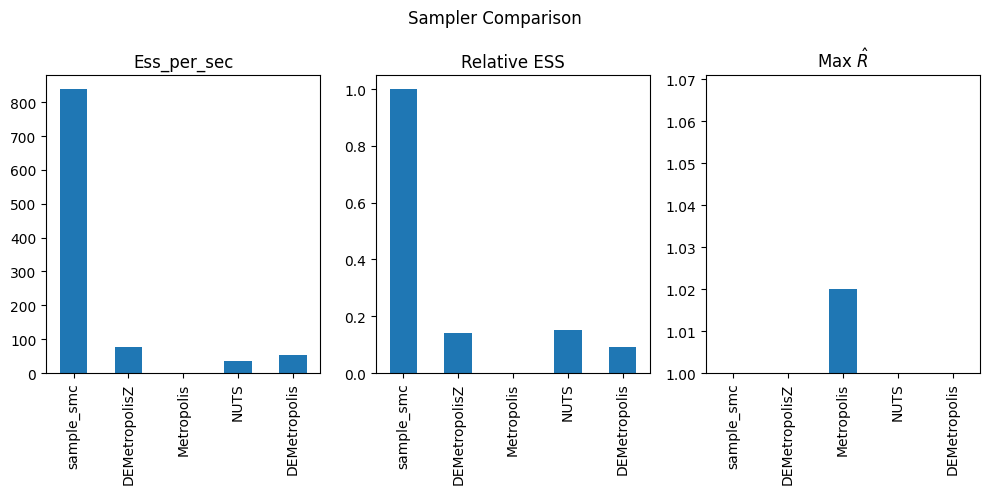
\includegraphics[width=0.9\linewidth, height = 0.5\linewidth]{Figures/Result_Model1/best_res_Ess_Rel_Ess_Rhat_without_init.png}
    \caption{Bar plots comparison of the Ess per time execution(left), the ESS per draws or Relative ESS (middle) and the maximum $\hat{R}$(right)}
    \label{fig:SIR_Bar_plot_Comparison}
\end{figure}
\begin{table}[H]
    \centering
    \resizebox{\textwidth}{!}{%
    \begin{tabular}{|>{\centering\arraybackslash}p{0.06\linewidth}|l|l|l|l|l|l|l|l|l|l|l|} \hline 
    &Param&  Mean & sd & hdi $ 3\%$ & hdi $97\%$ & \  mcse mean &mcse sd & Ess bulk &Ess tail & \  $\hat{R}$ \\ \hline 
    
    \multirow[t]{2}{*}{SMC} & $\beta$ & 0.20260& 0.00692 &0.18983& 0.21563 & 0.00042 & 0.00031 & 9611.78 & 10137.91 & 1.0248\\  
    & $\gamma$ &0.14542 & 0.00676 & 0.13317 & 0.15810 & 0.00041 & 0.00027 & 9069.01 & 9011.37 & 1.0246\\ \hline 

    \multirow[t]{2}{*}{NUTS} & $\beta$ & 0.20300 & 0.00700 & 0.18900	& 0.21600 & 0.00000 & 0.00000 & 6103.00	& 7433.00 &	1.0000\\ 
    & $\gamma$ & 0.14500 & 0.00700 & 0.13200 & 0.15800 & 0.00000 & 0.00000 & 6126.00 & 7274.00 & 1.0000 \\ \hline 
    
    \multirow[t]{2}{*}{DEM} & $\beta$ & 0.20222 & 0.00810 & 0.18736 & 0.21600 & 0.00028 & 0.00020 & 6397.74 & 8003.48 & 1.0017\\   
    & $\gamma$ & 0.14507 & 0.00832 & 0.13092 & 0.15844 & 0.00028 & 0.00020	& 6407.92 & 8043.05 & 1.0017\\ \hline  
% \cline{1-12}
    \multirow[t]{2}{*}{DEMZ} & $\beta$ &0.20233 & 0.00700 & 0.18955&0.21579 & 0.00000 & 0.00000 & 5257.94 & 6551.73 & 1.0000\\   
    & $\gamma$ &0.14504 & 0.00700 &0.13292 & 0.15820 & 0.00000 & 0.00000 &5260.64 & 6582.31 & 1.0000\\ \hline  
% \cline{1-12}\\
    \multirow[t]{2}{*}{ MH}& $\beta$ & 0.20883 & 0.02946 &0.18368 & 0.24388 & 0.00682 & 0.00491 & 46.45& 39.95 & 1.1030\\  
    &$\gamma$ & 0.15187 & 0.02943 & 0.12735 & 0.18591 & 0.00675 & 0.00487 & 46.44 & 40.41 & 1.1031\\ \hline
    \end{tabular}
    }%
    \caption{Metric mean summary over $100$ runs}
    \label{tab:SIR_Summarize_mean}
\end{table}
\subsection{SEIR age-stratified model}
In this experiment, the problem dimension is $d=16$. To minimize fluctuations in the data fitted to our model, we applied a $14$-point rolling mean. Due to the simplicity of our model, we focused on the outbreak period from August 2020 to November 2020, during which the data exhibits a nearly bell-shaped curve. 
We run the sampling algorithms with a sufficient number of draws and tuning (see Table (\ref{tab:SEIR_performance_metrics})).

As observed in Table (\ref{tab:SEIR_performance_metrics}), increasing the dimensionality of the problem leads to higher computation times for the algorithms. Specifically, the NUTS algorithm exhibits significantly longer computation times compared to other samplers, despite requiring only half the number of draws. However, as shown in Figure (\ref{fig:SEIR_Bar_plot_Comparison}), NUTS achieves superior performance metrics, including the highest ESS and relative ESS, along with the lowest $\hat{R}$ statistic.  

The Figure (\ref{fig:SEIR_fitting_test}) shows a comparison between model estimated counted COVID-19 cases  through each sampler against the observed data. Again the NUTS followed by the SMC are seamless more accurate in term of finding the best fit.

The maximum likelihood estimates(MLE) of the transmission rates by each sampler are plotted in Figure(\ref{fig:SEIR:transm_rate_estim_by_sampler}). Firstly, this figure illustrates how our model reveals differences in transmission rates across age groups. The variation between values obtained using different samplers indicates significant uncertainty in estimating the corresponding parameters. The dispersion of these estimated parameters is somewhat consistent with the age-related factors in transmission dynamics in England during the observed period, as evidenced by the dispersion of observed cases across age groups in Figure(\ref{fig:total_case_UK}).  
\begin{table}[H]
    \centering
    \caption{Summary of sampler performance metrics}
    \resizebox{\textwidth}{!}{%
    \begin{tabular}{|c|c|c|c|c|c|c|c|c|}
         \hline
         Samplers & Draws & Chains & Tune & Time (S) & Mean ESS & Min ESS & ESS/Second & Max $\hat{R}$ \\
         \hline
         SMC & 40000 & 4 & 0 & 417.1 & 121799.42&	17507.09& 52.25 & 1.000466\\ \hline 
         MH & 40000 & 4 & 5000 & 2677.5 &19573.30&7823.89 &7.31 & 1.000607 \\ \hline 
         DEMZ & 40000 & 4 & 5000 & 358.5 & 1806.079& 1048.13&	5.03&1.011844 \\ \hline 
         DEM & 40000 & 4 & 5000 & 504.6 & 879.91&477.61&	1.74& 1.008854 \\ \hline
         NUTS & 20000 & 4 & 2000 & 5936.08 & 68124.63&51458.69&11.48& 1.000321 \\
         \hline
    \end{tabular}
    }%
    \label{tab:SEIR_performance_metrics}
\end{table}
\begin{figure}[H]
    \centering
    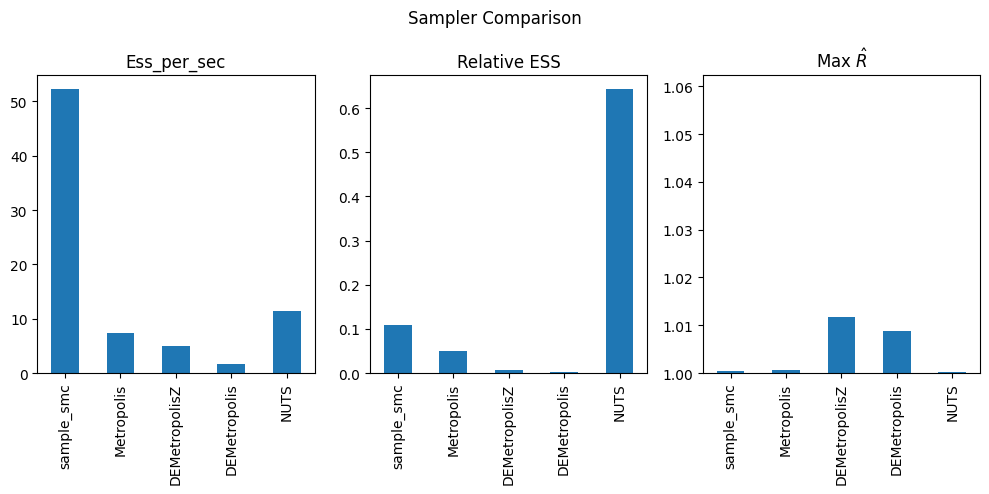
\includegraphics[width=0.9\linewidth, height = 0.5\linewidth]{Figures/Model_2/SEIR_bar_comparison.png}
    \caption{SEIR age-stratified: Bar plots comparison of the Ess per time execution(left), the ESS per draws or Relative ESS (middle) and the maximum $\hat{R}$(right)}
    \label{fig:SEIR_Bar_plot_Comparison}
\end{figure}

\begin{figure}[H]
    \centering
    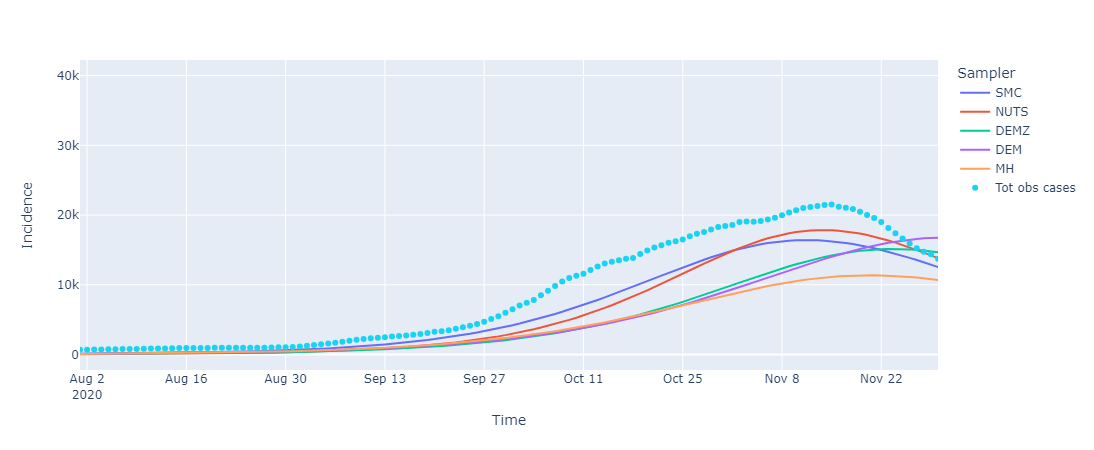
\includegraphics[width=0.9\linewidth, height = 0.5\linewidth]{Figures/Model_2/fitting_test.png}
    \caption{SEIR-age-stratified: Model fitting test by each sampler. Total cases in England Aug 2020 to Nov 2020}
    \label{fig:SEIR_fitting_test}
\end{figure}

\begin{figure}[H]
    \centering
    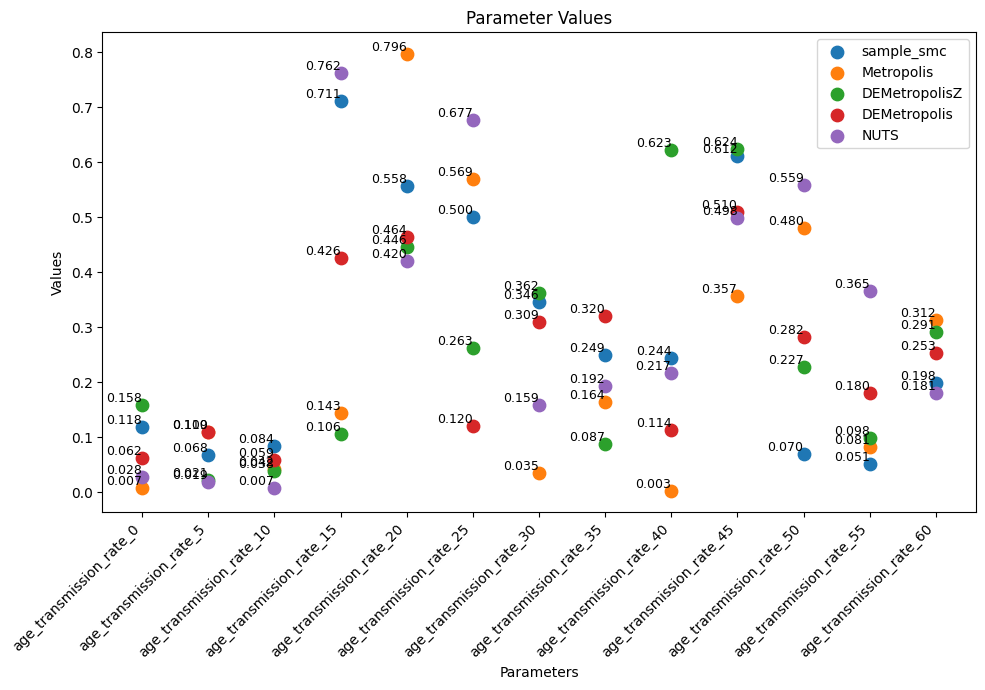
\includegraphics[width=0.9\linewidth]{Figures/Model_2/transm_rate_estim_by_sampler.png}
    \caption{SEIR model transmission rate estimation by different samplers}
    \label{fig:SEIR:transm_rate_estim_by_sampler}
\end{figure}
\subsubsection{Reverse Engineering}
In this particular experiment, we are able to characterise a nearly "true" convergence since our posterior distribution is well-known. We compute the Kullback-Leibler divergence(as implemented in \href{https://docs.scipy.org/doc/scipy/reference/generated/scipy.special.kl_div.html#scipy.special.kl_div}{\textcolor{blue}{Scipy}}) between the true posterior and the distribution obtain by the MCMC sampler. 
We mainly experimented two scenario:
\begin{itemize}
    \item A posterior distribution with a large gap between modes;
    The complex shape of this posterior distribution often complicates the sampling process. Our experiments demonstrate that the algorithm may fail to sample effectively from such distributions, despite being designed to handle these challenges. The Figure \ref{fig:pseudo_convergence},  illustrates the pseudo-convergence phenomenon occurring while using DEMZ. The rank plot of the chains shows a good mix indicating a satisfactory $\hat{R}$ statistic value. The algorithm performed an effective sample size of $9,360$ in 131 seconds with $10,000$ draw per chain.
    \item A posterior distribution with slight overlap between the two mixed Gaussian distributions:
Overall, in terms of $\hat{R}$ and ESS statistics, the SMC sampler outperforms the others, as shown in Figure \ref{fig:Reverse_Engi_Bar_plot}. However, while NUTS yields the best Kullback-Leibler divergence (KL\textunderscore div) value, it underperforms in other convergence diagnostics. 

In figures \ref{fig:pseudo_convergence} and \ref{fig:rank_plot_pseudo_conv_DEMZ}, we illustrate the pseudo convergence by the DEMz while sampling from a bimodal posterior distribution of $\beta$ with sever between trough modes. $\hat{R} < 1.01$). Draws = $10,000$ per chain and Tune = $1,000$.

In the other hand, the figure(\ref{fig:Posterior-density-compar}) is a comparison of the true posterior density against the one obtain by each algorithm.
\end{itemize}
\begin{figure}[h]
    \centering
    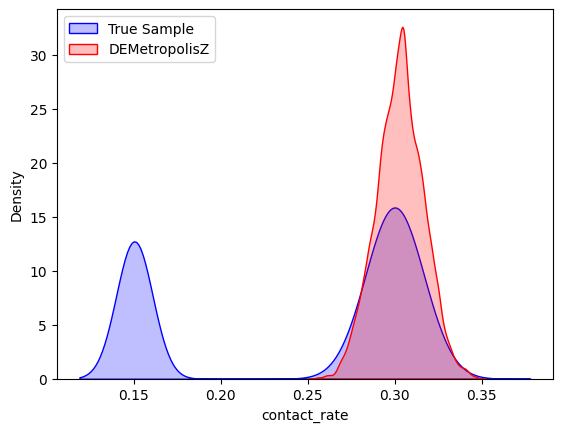
\includegraphics[width=0.5\linewidth]{Figures/Reverse-Ingineering/pseudo_convergence.png}
    \caption{Posterior density comparison of the DEMZ against true posterior}
    \label{fig:pseudo_convergence}
\end{figure}%

\begin{figure}[h]
    \centering
    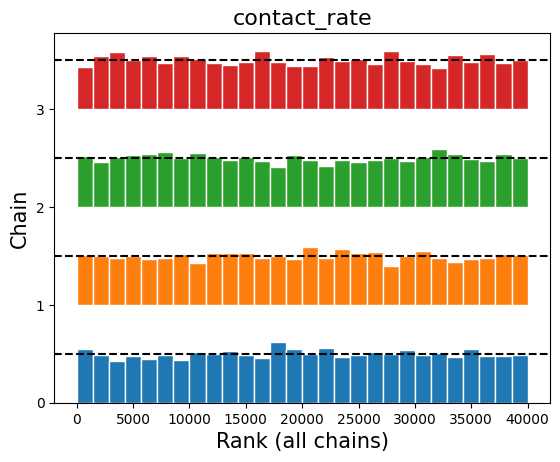
\includegraphics[width = 0.5\linewidth]{Figures/Reverse-Ingineering/rank_plot_in_pseudo_convergence_DEMz.png}
    \caption{Chains rank plot}
    \label{fig:rank_plot_pseudo_conv_DEMZ}
\end{figure}

%\caption{Illustration of pseudo convergence by the DEMz while sampling from a bimodal posterior distribution of $\beta$ with sever between trough modes. $\hat{R} < 1.01$). Draws = $10,000$ per chain and Tune = $1,000$}
    
%\end{figure}
\begin{figure}[H]
    \centering
    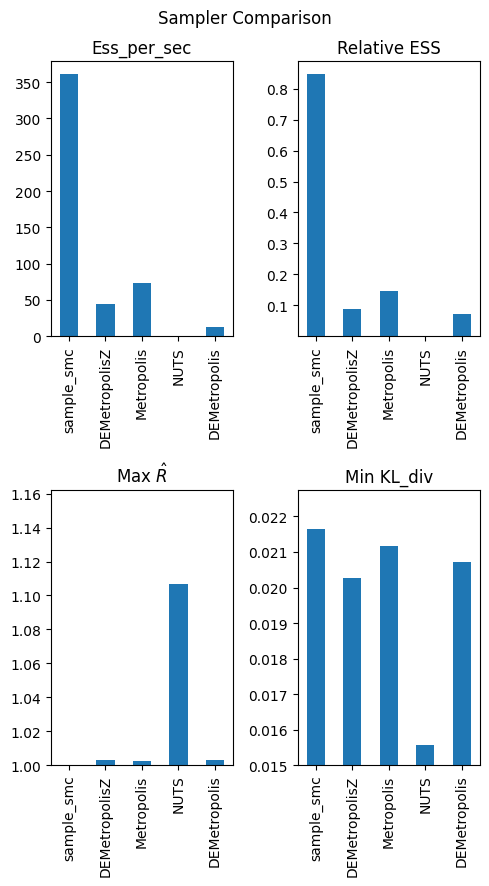
\includegraphics[width=0.7\linewidth]{Figures/Reverse-Ingineering/plot_bars_comparison_2.png}
    \caption{Bar plot comparison of sampler. After $100$ runs, we select the inference data corresponding to the minimum value of the Kullback-Leibler divergence}
    \label{fig:Reverse_Engi_Bar_plot}
\end{figure}

\begin{figure}
    \centering
    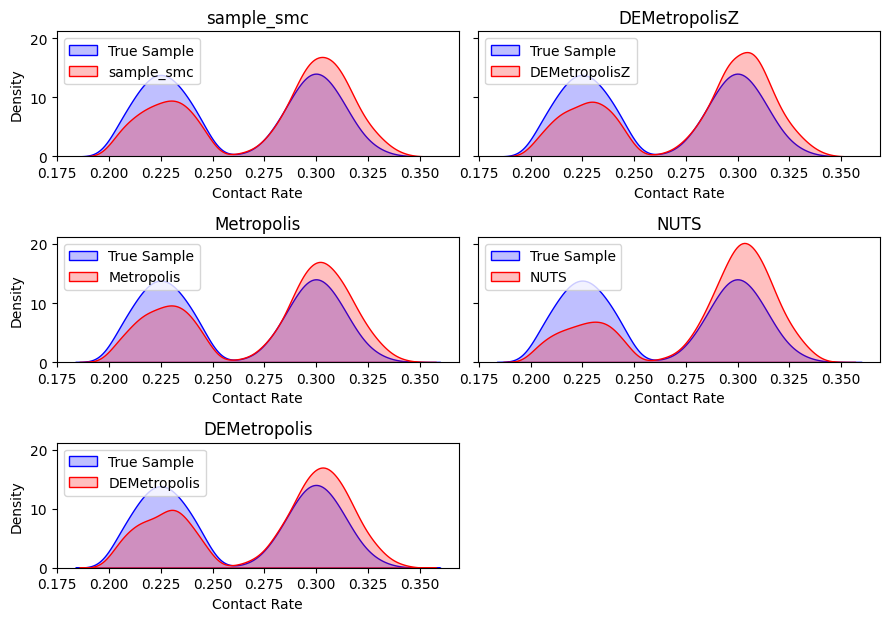
\includegraphics[width=0.9\linewidth]{Figures/Reverse-Ingineering/Multi_run_all_posterior_plot.png}
    \caption{Posterior density comparison of Bayesian algorithms samples against the true posterior. The plotted posteriors correspond to the minimum value of the KL\textunderscore div across 100 simulation for each sampler }
    \label{fig:Posterior-density-compar}
\end{figure}

\begin{table}[H]
    \centering
    \begin{tabular}{|c|c|} \hline 
         Samplers& Mean times (S)\\ \hline 
         SMC& 87.624336
\\ \hline 
         DEM& 229.900158
\\ \hline 
         DEMZ& 78.724631
\\ \hline 
         MH& 79.279480\\ \hline 
         NUTS& 582.967062\\ \hline
    \end{tabular}
    \caption{Algorithm mean time executions comparison after 100 runs }
    \label{tab:Reverse_Time_execution}
\end{table}

\subsection{Discussion}
Our study primarily demonstrates how the performance of Bayesian sampling algorithms can vary slightly depending on the specific problem at hand. Although convergence diagnostics for inferring parameters in ODE-based infectious disease models can be complex, utilizing automatic parameter tuning tools in PyMC and Numpyro helps abstract away some of the complexities associated with each sampling algorithm. This approach facilitates more effective and reliable sampling across different models. 


The results should be evaluated in relation to our model hypothesis, as the convergence of algorithms depends significantly on the model’s ability to fit the observations, the chosen target distribution, and the starting conditions.

The reverse engineering experiment revealed sub-optimal performance of the NUTS, which can be attributed to several factors: the uniform initialization strategy within the interval 
$[-2,2]$(NUTS default initialisation) and challenges related to using NUTS effectively alongside SUMMER with auto-differentiation techniques. 

The observed pseudo-convergence phenomenon underscores that sampler can fail to fully explore the true posterior, especially when the posterior distribution exhibits severe multi-modality. In in this case we can not typically rely on classical MCMC convergence diagnostics such as the $\hat{R}$ statistics. Performing a landscape analysis of the posterior before the sampling phase could provide valuable insights for configuring algorithms more effectively. Using estimated parameter from a sub-space of the posterior could be misleading in ID modelling for instance in term of predicting or estimating interventions effects. 

In the other hand, the results we obtain through the SEIR age-stratified model using different algorithms reveal that our model can capture the observation data but most importantly depicted the variability in parameter estimate with respect to the involved algorithm.

Overall, aside from cases involving bimodal posterior distributions, NUTS demonstrates strong performance. However, SMC methods can serve as an effective alternative, especially when auto-differentiation computations are prohibitive.

\newpage


%\nocite{*}
\bibliographystyle{plain}
\bibliography{references}
\end{document}
